
\documentclass[11pt]{article}
\usepackage[margin=1in]{geometry}
\usepackage{graphicx}
\usepackage{float}
\usepackage{amsmath}
\usepackage{booktabs}
\usepackage{hyperref}
\usepackage{xcolor}

\definecolor{alertred}{RGB}{220,53,69}
\definecolor{successgreen}{RGB}{40,167,69}

\title{Enhanced Exposure Validation Report\\
\large Comprehensive Analysis of OR vs AND Logic}
\author{Ryhan Suny\\Toronto Metropolitan University}
\date{May 25, 2025}

\begin{document}
\maketitle

\section{Executive Summary}

This report presents a comprehensive analysis comparing OR logic (any criterion) versus AND logic (all criteria) for SSD exposure definition. The analysis reveals a 722-fold difference in exposed population size with significant implications for study power and validity.

\section{Key Findings}

\subsection{Population Impact}

\begin{table}[H]
\centering
\begin{tabular}{lccc}
\toprule
\textbf{Metric} & \textbf{OR Logic} & \textbf{AND Logic} & \textbf{Ratio} \\
\midrule
Exposed Patients & 143,579 & 199 & 722:1 \\
Percent Exposed & 55.9\% & 0.1\% & - \\
Minimum Detectable Effect & 0.008 & 0.198 & - \\
\bottomrule
\end{tabular}
\caption{Comparison of exposure definitions}
\end{table}

\begin{figure}[H]
\centering
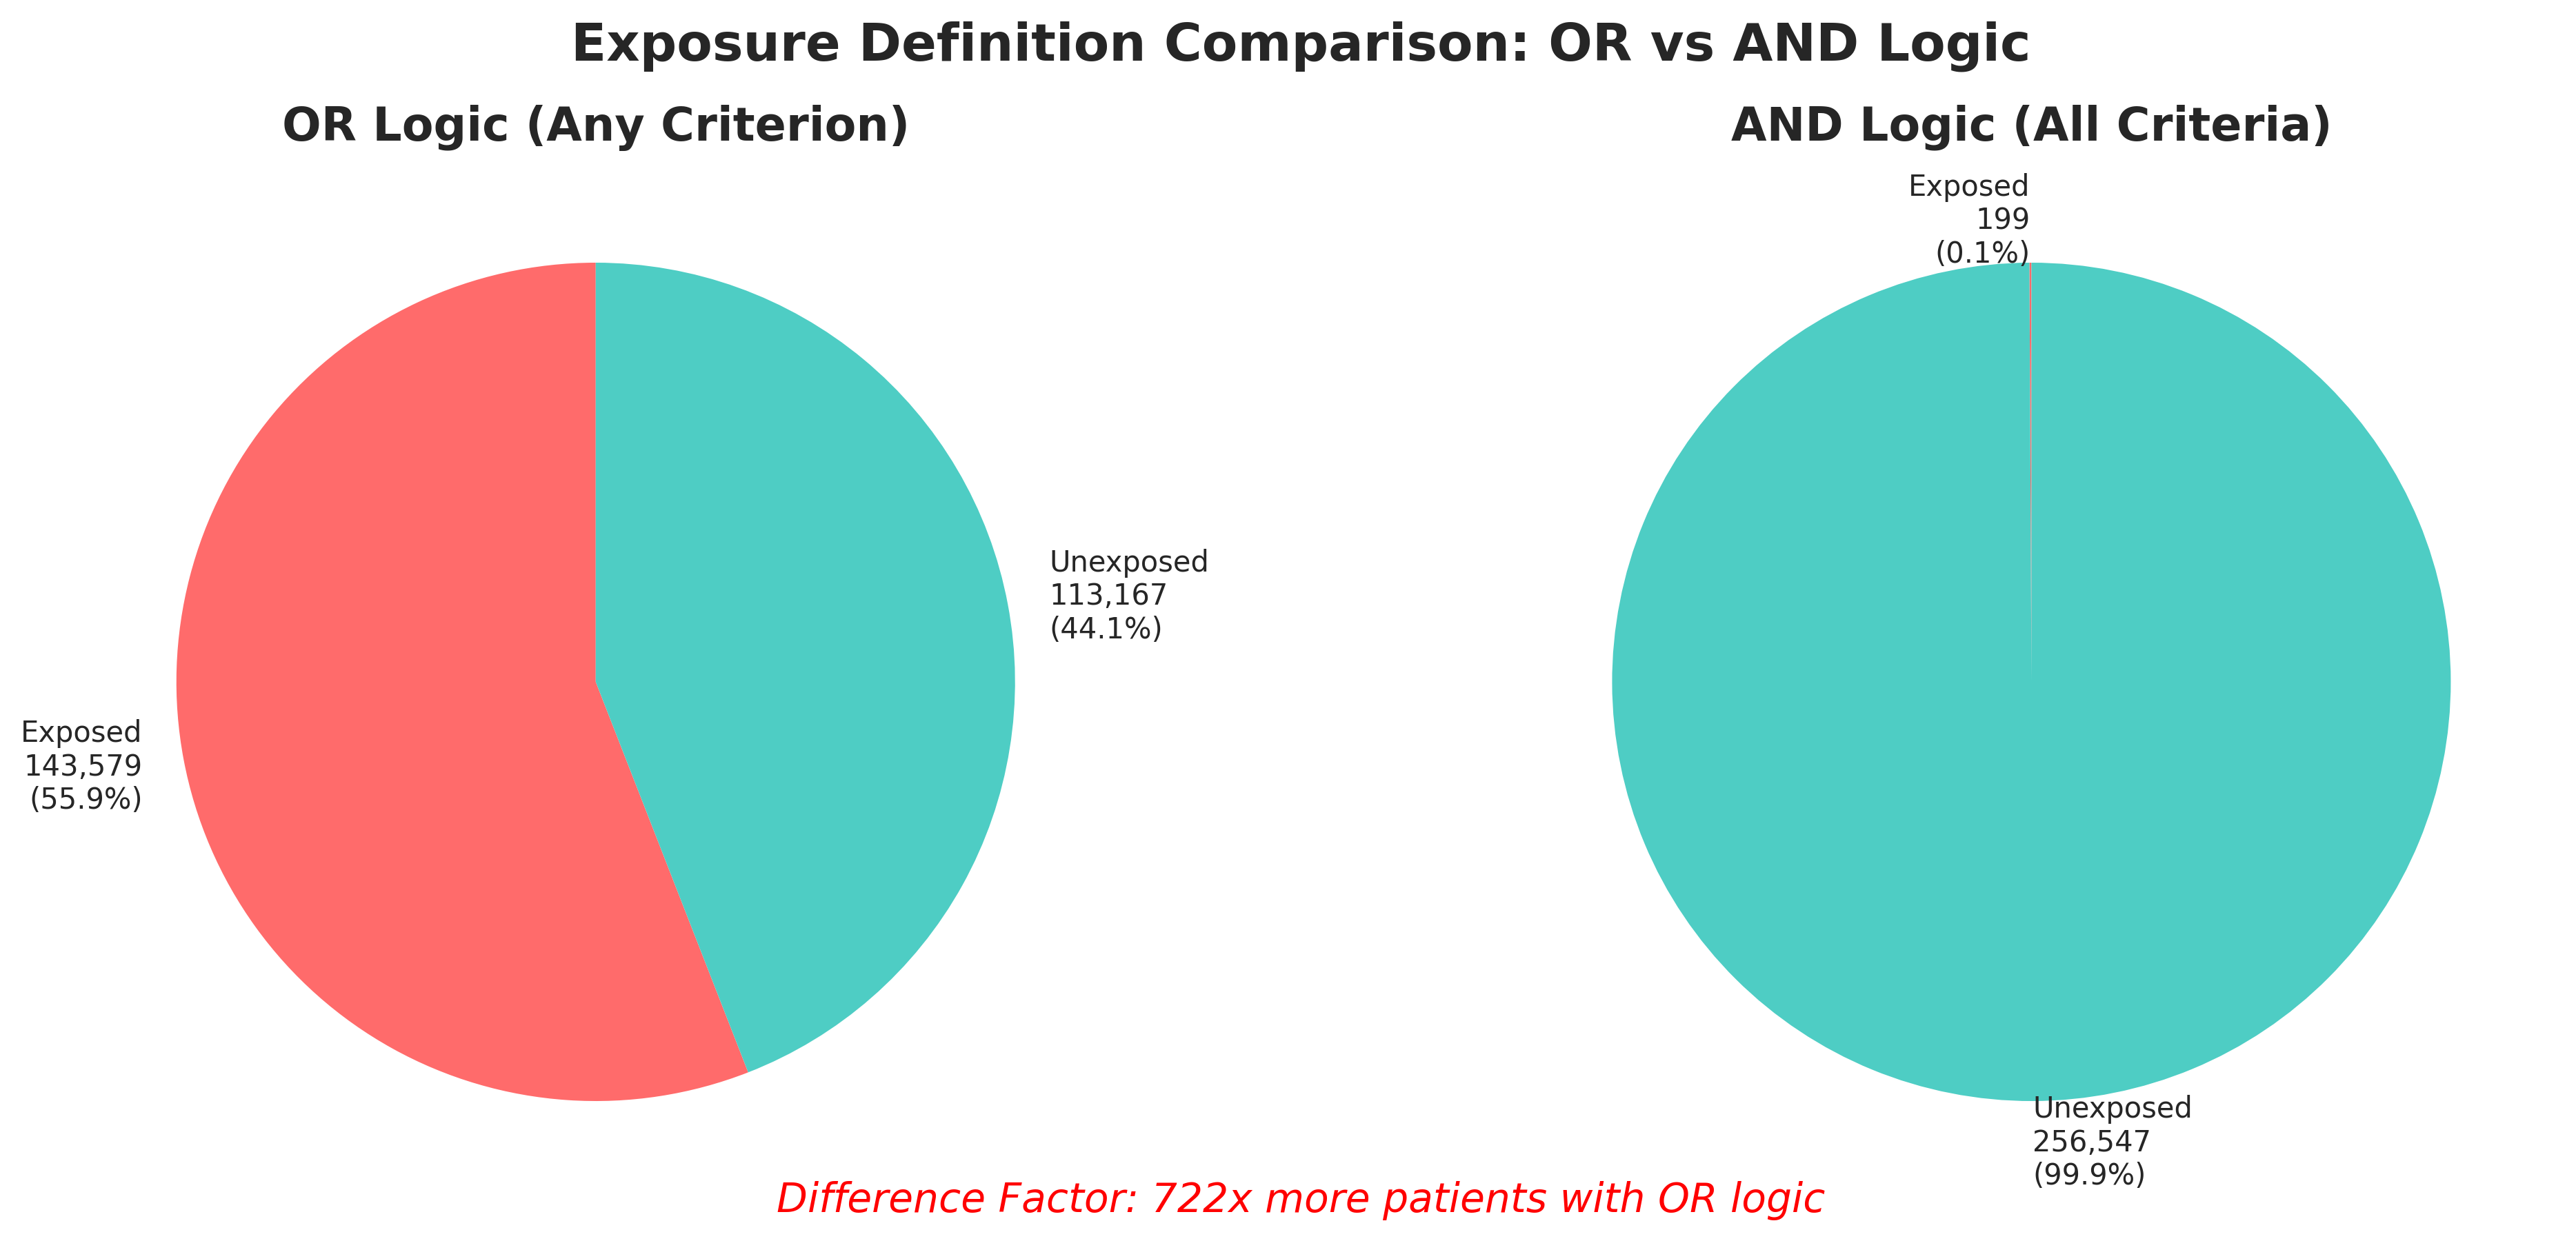
\includegraphics[width=0.9\textwidth]{exposure_comparison.png}
\caption{Visual comparison of OR vs AND logic exposure rates}
\end{figure}

\subsection{Criteria Overlap Analysis}

\begin{figure}[H]
\centering
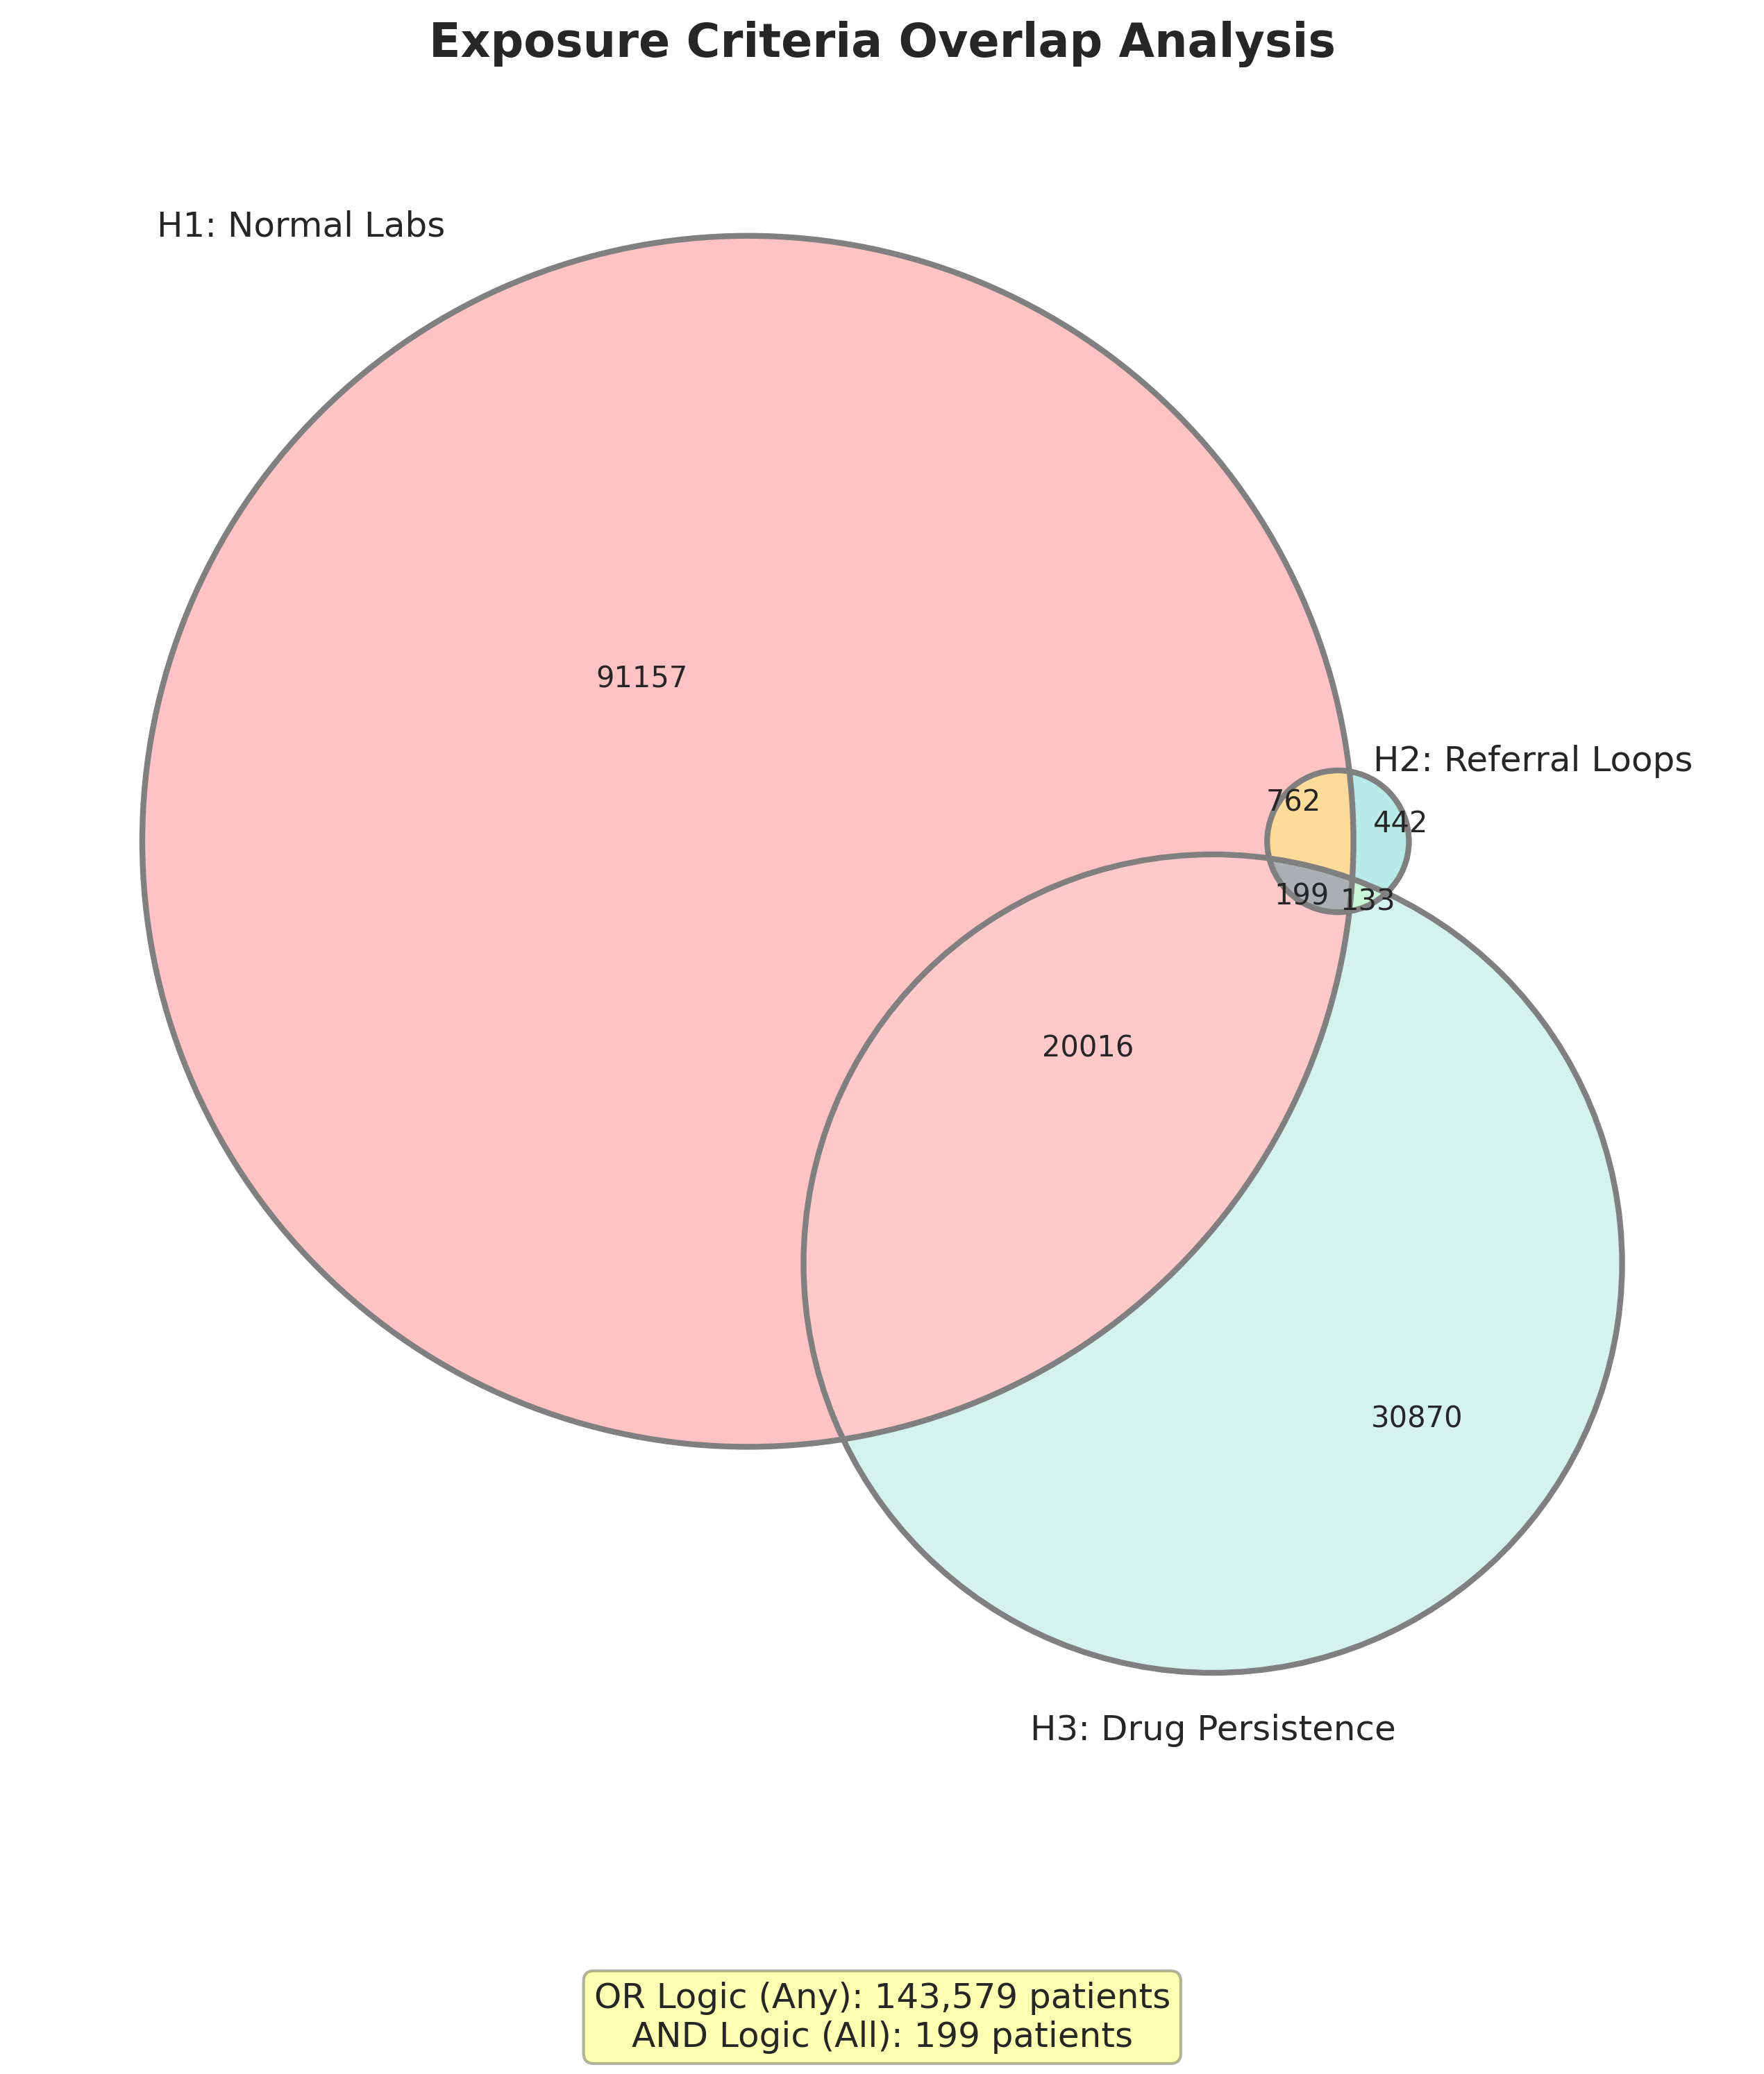
\includegraphics[width=0.8\textwidth]{criteria_venn_diagram.png}
\caption{Venn diagram showing overlap between exposure criteria}
\end{figure}

The overlap analysis reveals:
\begin{itemize}
\item Only 199 patients meet all three criteria
\item 143,579 patients meet at least one criterion
\item Substantial heterogeneity exists in criterion combinations
\end{itemize}

\subsection{Demographic Differences}

\begin{figure}[H]
\centering
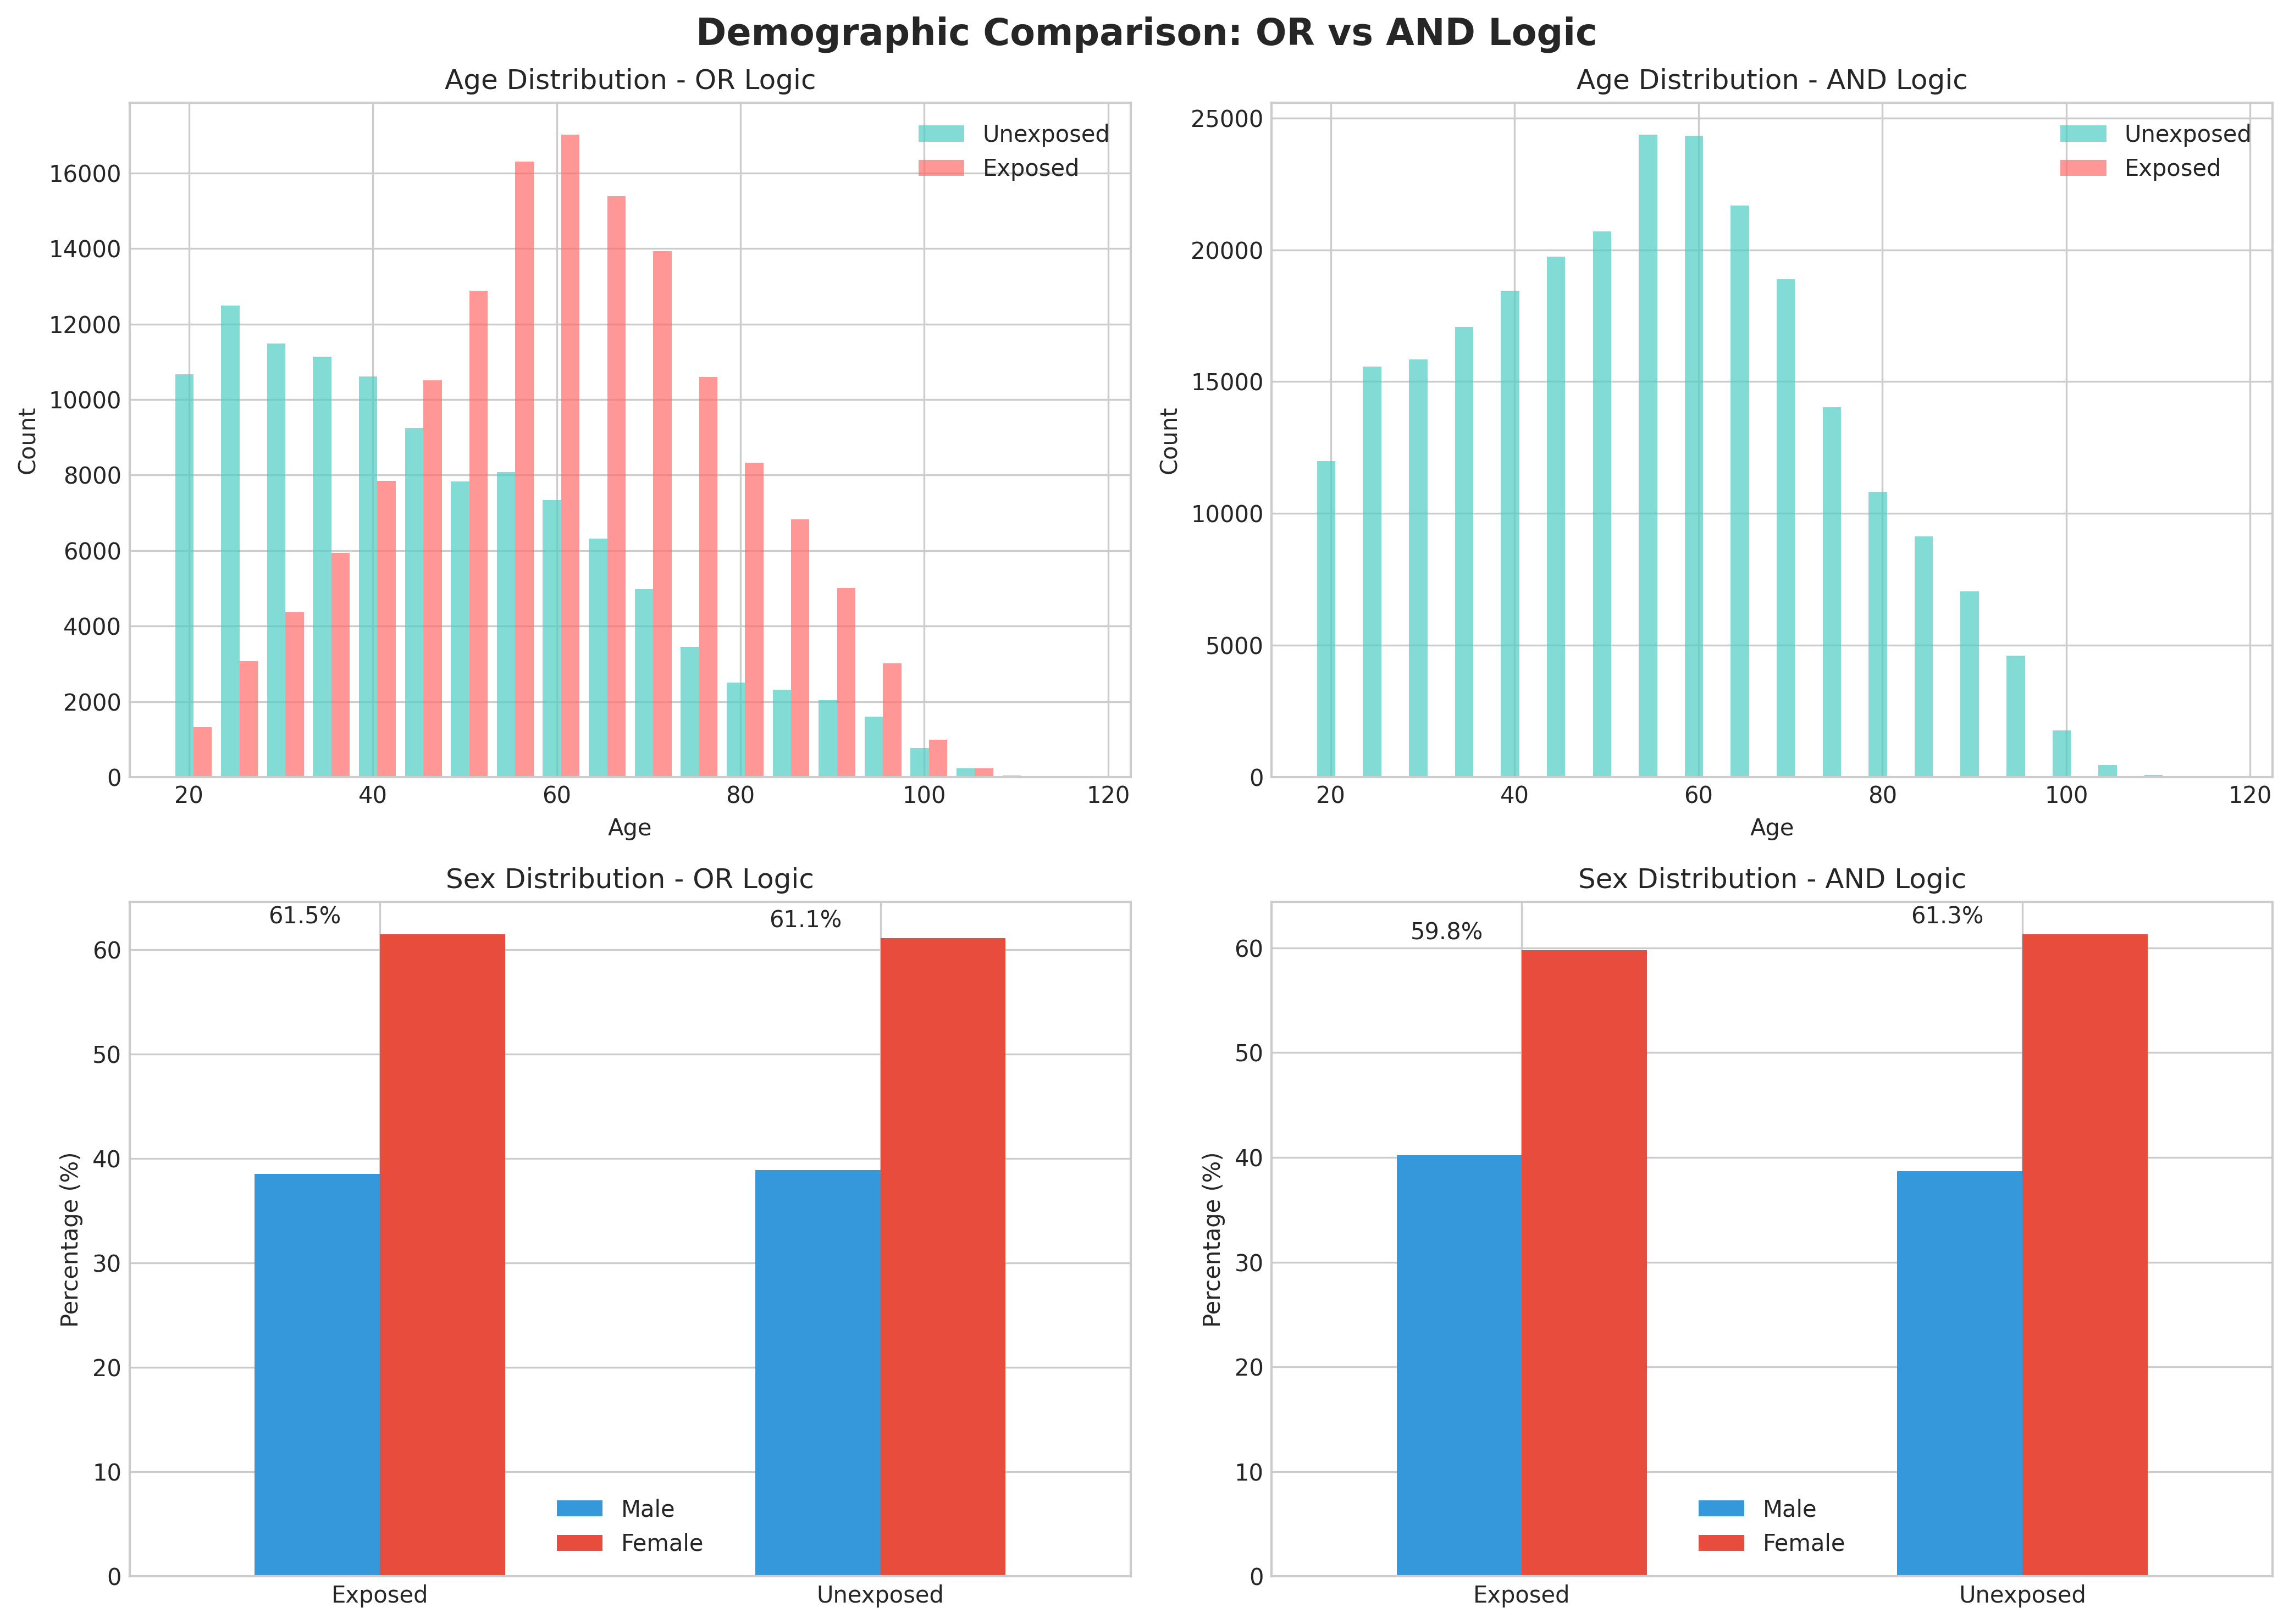
\includegraphics[width=\textwidth]{demographic_comparison.png}
\caption{Demographic characteristics by exposure definition}
\end{figure}

\subsection{Statistical Power Analysis}

\begin{figure}[H]
\centering
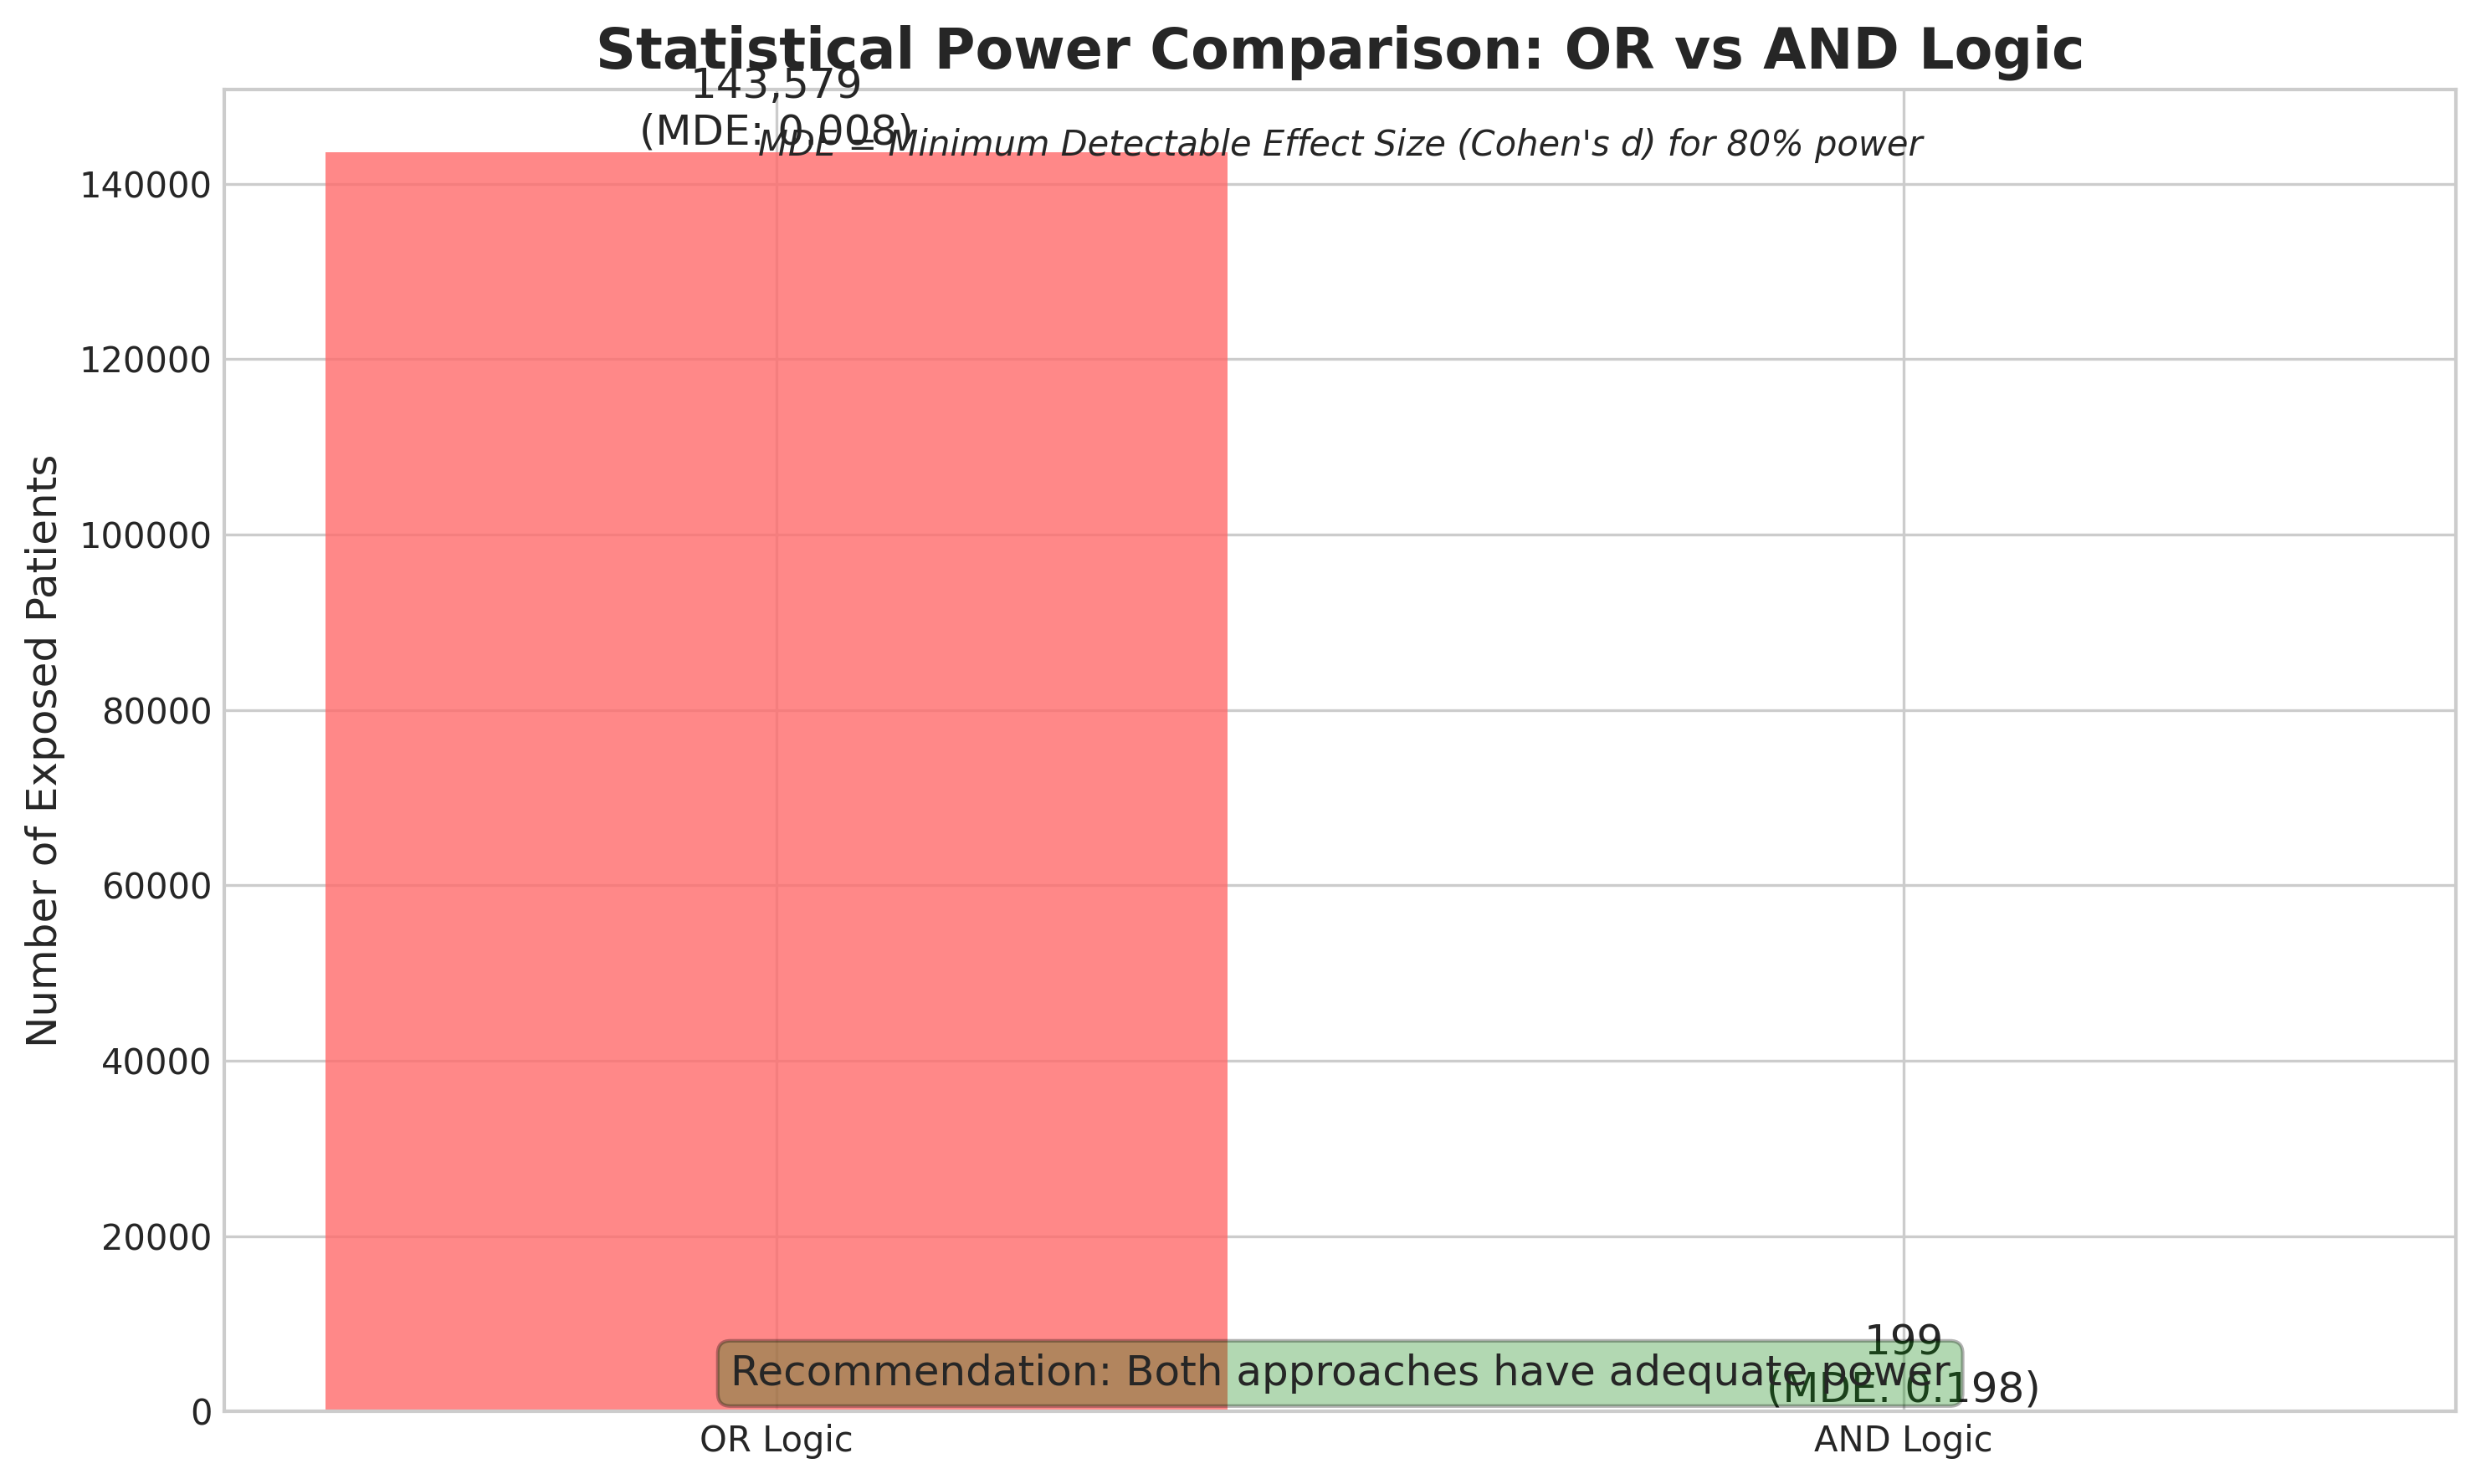
\includegraphics[width=0.8\textwidth]{power_analysis_comparison.png}
\caption{Statistical power comparison between approaches}
\end{figure}



\subsection{Criteria Intensity}

\begin{figure}[H]
\centering
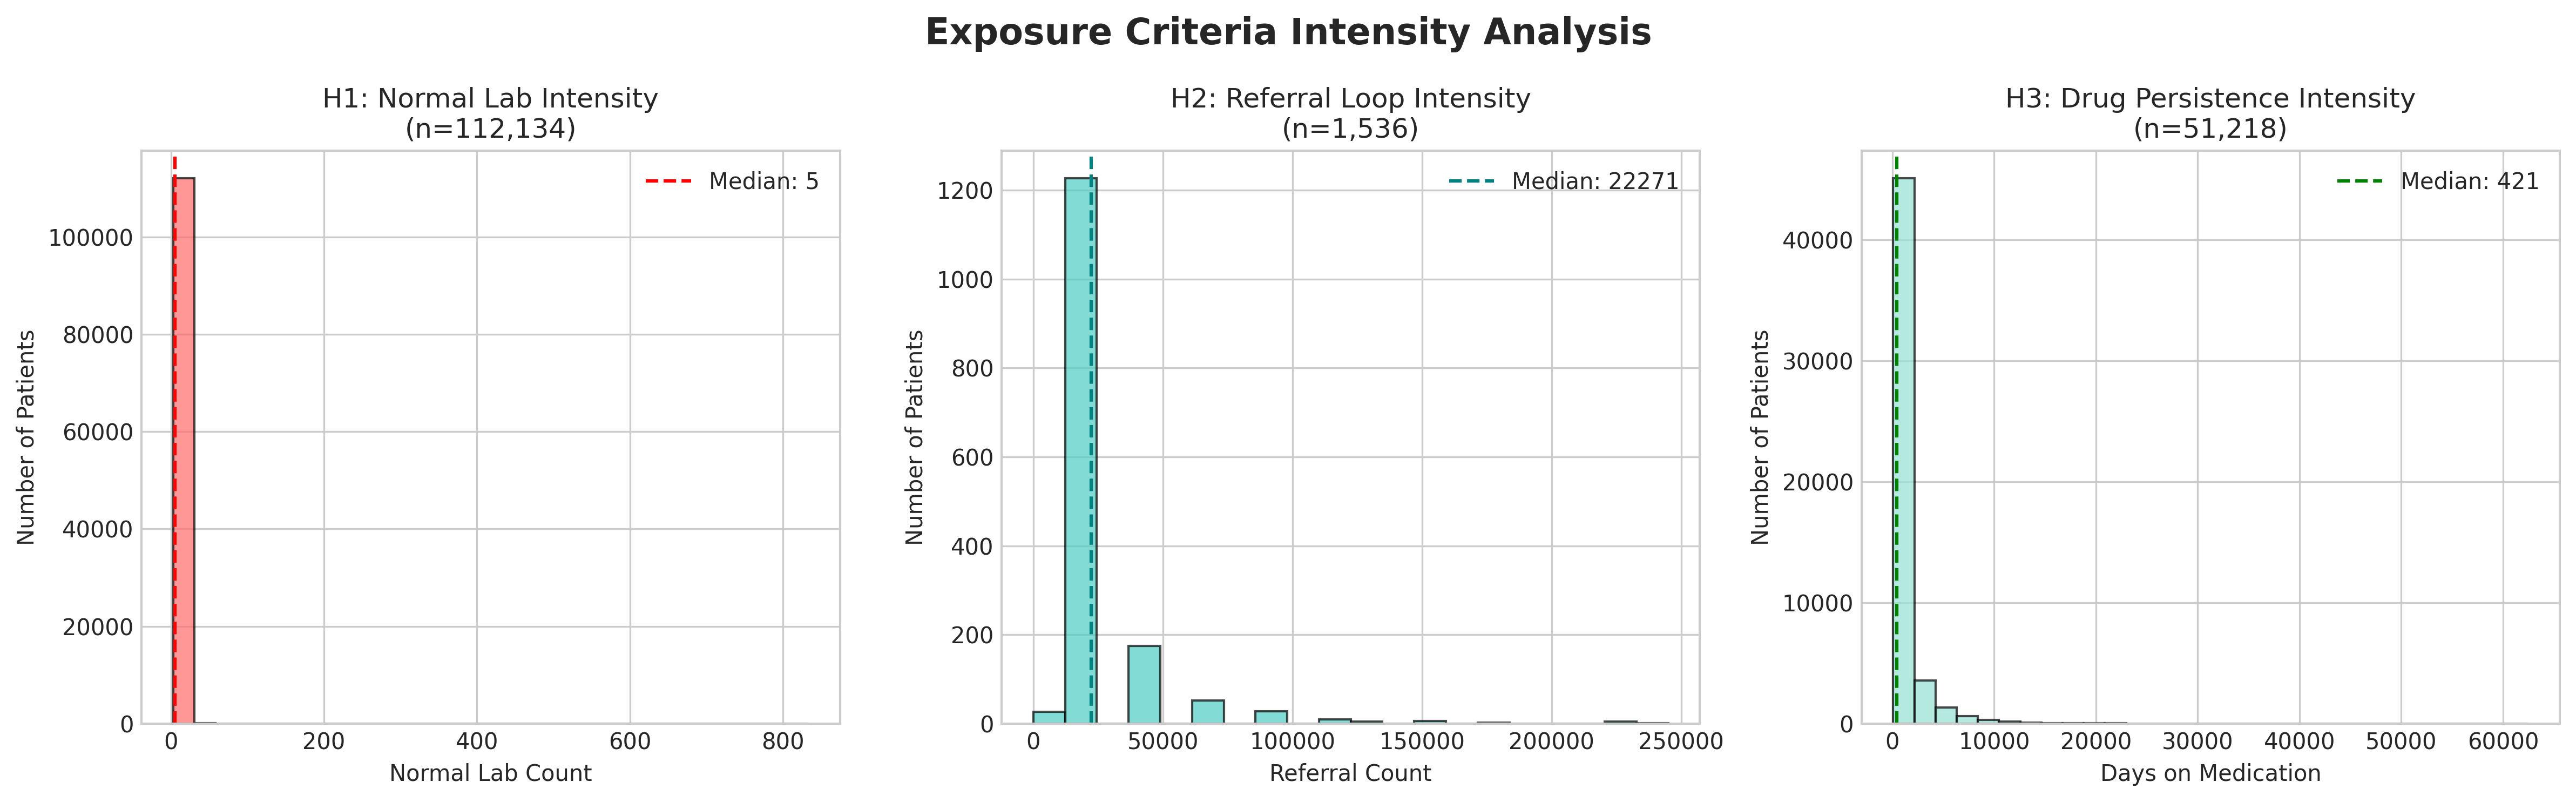
\includegraphics[width=\textwidth]{criteria_intensity.png}
\caption{Distribution of criterion intensity measures}
\end{figure}

\section{Recommendations}

Based on the comprehensive analysis:

\begin{enumerate}
\item \textbf{Primary Analysis}: Either approach viable depending on clinical priorities
\item \textbf{Power Consideration}: Both approaches have adequate power
\item \textbf{Clinical Validity}: AND logic provides more specific phenotype but limited sample
\end{enumerate}

\section{Conclusion}

The choice between OR and AND logic represents a fundamental trade-off between statistical power and clinical specificity. The AND logic identifies a highly specific but extremely small cohort, while OR logic provides adequate power but may include heterogeneous phenotypes.

\end{document}
